\documentclass[11pt,fleqn]{report}

\usepackage{../../fancyStructure}
%\usepackage{libertine}
%\usepackage{libertinust1math}
%\usepackage[T1]{fontenc}

\tikzset{>=latex}

\newcommand{\contract}{\boldsymbol{\lrcorner}\, }

\begin{document}
	
\title{General Relativity - Part III}
\author{Sam Crawford}

\maketitle
\tableofcontents
\listoftodos

\chapter{Manifolds}

General relativity is, simplifying somewhat, a condition on the curvature of a pseudo-Riemannian manifold. I will not include a definition of a manifold here, other than to say it is a topological space which is locally diffeomorphic to $\mathbb{R}^n$, where $n$ is the dimension of the manifold.

\section{Curves, Vector Fields \& Tensors}

As with any treatment of manifolds, one of the major goals of GR is to be able to compare tangent vectors at different points.\footnote{Specifically in order to establish \textit{parallel transport} of $4$-velocities along geodesics.}
First, however, we should probably begin by actually defining a tangent vector.

\begin{definition}
A \textbf{smooth curve} $\gamma$ is a smooth map \begin{equation}
\gamma : [-1,1] \to U \subset M.
\end{equation}
If $U$ admits a local chart, $\phi$, we can define $\gamma: \epsilon \to \gamma^\mu(\epsilon)$ such that $\gamma^\mu = r^\mu\circ\phi\circ\gamma$.
\end{definition}
We may ask ourselves then, what does it mean to differentiate $\gamma$? Without thinking about it too much, it is intuitive to write \begin{equation}
v = \left. \frac{d\gamma}{d\epsilon} \right\vert_{\epsilon = 0}.
\end{equation}
Indeed, this makes perfect sense if $M \subset \mathbb{R}^n$, as $\gamma$ is a vector. Furthermore, we can visualise $v$ as being a vector 'tangent' to the manifold at $\gamma(0)$.

\paragraph{} However, there is a more useful understanding. Recall that for a scalar field $f: \mathbb{R}^n \to \mathbb{R}$, we can define the \textbf{directional derivative} along a vector $\mathbf{x}$ at the point $p$ as
	\begin{equation}
		\nabla_\mathbf{x} f (p) \coloneqq \lim_{\epsilon \to 0} \frac{
			f(p + \epsilon \mathbf{x}) - f(p)
		}{
			\epsilon
		} = \mathbf{x} \cdot \boldsymbol{\nabla}f(p).
	\end{equation}
This notion generalises quite well to the manifold case. The curve $\gamma$ provides a direction along which we can take derivatives

\subsection{Covectors}

\begin{definition}
Let $E$ be a real vector space. The \textbf{dual space} to $E$, denoted $E^*$, is the vector space of linear maps $f:E\to\mathbb{R}$
\end{definition}

\paragraph{}For any finite dimensional vector space $E$, it can easily be shown that $\textrm{dim}(E) = \textrm{dim}(E^*) $, but there exists \textit{no} basis independent (natural) isomorphism between the two spaces. Given a choice of basis $\{\mathbf{e}_i\}_{i=1}^{n}$ for an $n$-dimensional vector space $E$, one can define the \textbf{dual basis} $\{f^i\}_{i=1}^n$ by \begin{equation}
f^i(\mathbf{e}_j) = \delta^i_j.
\end{equation}
So for any general vector $v =  v^i \mathbf{e}_i$, we have $f^i(v) = v^i$.

\paragraph{}Fortunately, we \textit{can} define a natural isomorphism between $E$ and $\left(E^*\right)^*$ by \begin{eqnarray}
\phi : E \to \left(E^*\right)^*, & x \mapsto \phi_x ,& \phi_x(f) = f(x).
\end{eqnarray}

\begin{definition}
A  \textbf{covector} is an element of $T_pM^*$, i.e. a linear map $T_pM \to \mathbb{R}$. The space of all such maps at a point is called the \textbf{cotangent space}, and the disjoint union thereof is the \textbf{cotangent bundle}, $TM^*$. A \textbf{1-form} is a section of the cotangent bundle, $\omega \in \Gamma\left(TM^*\right) = \Omega^1(M)$.
\end{definition}

By convention, though it does have an intuitive meaning, we denote the dual of the basis $\{\left.\nicefrac{\partial}{\partial x^\mu}\right\vert_p \}$ by $\{\mathrm{d}x^\mu|_p\}$. We define the action of a 1-form on a vector field pointwise, so $\omega(X) : M \to \mathbb{R}$ ; $p \mapsto \omega|_p\left(X|_p\right)$. An alternative notation for this is the \textbf{contraction} of $\omega$ by $X$, written as $X \contract \omega$.

\paragraph{} We can use our intuition from changing variables in integration to derive the formula for the change of basis of $TM^*$. Let $(U,\phi),(V,\psi)$ be charts giving rise to coordinates $\{x^\mu\}$ and $\{y^\mu\}$ respectively, then \begin{equation}\label{ChangeDualBasis}
\mathrm{d}y^\mu = \left(\frac{\partial y^\mu}{\partial x^\nu}\right) \mathrm{d}x^\nu.
\end{equation}
If we say $\omega = \omega_\mu \mathrm{d}x^\mu = \widetilde{\omega}_\nu \mathrm{d}y^\nu$, inserting \eqref{ChangeDualBasis} into the second equation, then comparing coefficients, we see the resulting change in coordinate functions is \begin{equation}
\omega_\mu = \left(\frac{\partial y^\nu}{\partial x^\mu}\right) \widetilde{\omega}_\nu.
\end{equation}

\subsection{Abstract Index Notation (Penrose)}
\paragraph{}Whenever we use Greek indices, it is implicit that we are working in a particular coordinate basis. However, a lot of results we find are true in a more general case. The aim of abstract indices is to display results that are true in \textit{any} basis. It is essentially a notational 'trick' that (among other things) makes the isomorphism between a vector space and its dual appear natural.

\paragraph{} We use Latin letters as abstract indices. So in abstract index notation, a vector field is written $X^a$, and a 1-form $X_a$. Note the symbol doesn't matter, but the location of the index. Contractions can then also be written $X\contract W = X^a W_a$.

\subsection{Tensors}

\begin{definition}
A \textbf{tensor} of type $(r,s)$ at $p \in M$ is a multilinear map \begin{equation}
T: \underbrace{T^*_pM\times \cdots \times T_p^*M}_{r \text{ copies}} \times \underbrace{T_pM\times \cdots \times T_pM}_{s \text{ copies}} \to \mathbb{R}
\end{equation}
\end{definition}
\begin{remark}
If we identify $\phi_X \sim X$ (which is unavoidable in abstract indices) then we can happily say that a tangent vector is a type $(1,0)$ tensor, and a covector is a type $(0,1)$ tensor. In fact in abstract indices we can label a type $(r,s)$ tensor as \begin{equation}
T^{a_1 \cdots a_r}_{b_1 \cdots b_s},
\end{equation}
thus contraction a tensor with an arbitrary vector/covector is as easy as summing over repeated indices.
\end{remark}

\paragraph{}As with tangent vectors and covectors, we can define the vector space of type $(r,s)$ tensors at a point $p \in M$ (which has dimension $n^{r+s}$), then form a vector bundle over $M$, usually denoted $T^r_{\phantom r s}(M)$. A tensor field is then simply a smooth section of this bundle $T \in \Gamma\left(T^r_{\phantom r s}(M)\right)$.

\begin{definition}
We can define a \textbf{contraction} as a map from a type $(r,s)$ tensor to a type $(r-1,s-1)$ tensor in abstract indices by (for example)\begin{equation}
T^{ab}_{\phantom{ab}cde} \mapsto S^b_{\phantom a de} = T^{ab}_{\phantom{ab}ade}.
\end{equation}
\end{definition}

\begin{definition}
Given a type $(r,s)$ tensor, $T$, and type $(p,q)$ tensor, $S$, the \textbf{tensor product} is defined as, for $\omega_i \in T^*_pM$, $v_i \in T_pM$ \begin{equation}\begin{split}
\left( T \otimes S\right)(\omega_1, \cdots, \omega_{r+p},v_1,\cdots,v_{s+q}) &=\\
T(\omega_1,\cdots,\omega_r,v_1,\cdots,v_s)\cdot &S(\omega_{r+1},\cdots,\omega_{r+p},v_{s+1},\cdots,v_{s+q}).
\end{split} \end{equation}
Alternatively, in abstract indices this reads \begin{equation}
\left(T \otimes S\right)^{a_1\cdots a_r b_1 \cdots b_p}_{c_1 \cdots c_s d_1 \cdots d_q} = T^{a_1 \cdots a_r}_{c_1 \cdots c_s}S^{b_1 \cdots b_p}_{d_1 \cdots d_q}.
\end{equation}
\end{definition}

\paragraph{} We can also define some more complicated manipulations of tensors using abstract indices: \begin{itemize}
\item (Anti-)symmetrisation of a $(0,2)$ tensor T:\begin{align}
S(v,u) := \tfrac{1}{2} \left(T(v,u) \pm T(u,v)\right) & \Leftrightarrow & S_{ab} = \tfrac{1}{2}\left(T_{ab} \pm T_{ba}\right) = T_{(ab)},T_{[ab]}.
\end{align}
\item For a general $(r,s)$ tensor \begin{align}
T^{(ab)c\cdots}_{d\cdots} &= \tfrac{1}{2}\left( T^{abc\cdots}_{d\cdots} + T^{bac\cdots}_{d\cdots} \right),\\
T_{(a|bc|d)} &= \tfrac{1}{2} \left( T_{abcd} + T_{dbca}\right), \\
T^{\cdots}_{[a_1\cdots a_n]} &= \tfrac{1}{n!} \sum_\sigma \left(\mathrm{sgn}(\sigma)T^{\cdots}_{\sigma(a_1,\cdots ,a_n)}\right).
\end{align}
\item The \textbf{wedge product} of two covectors is the anti-symmetrisation of their tensor product\begin{align}
\omega \wedge \eta := \tfrac{1}{2}(\omega\otimes\eta-\eta\otimes\omega).
\end{align}
\item More generally, for a type $(0,s)$ tensor and type $(0,q)$, we can use abstract indices \begin{equation}
\left(\omega\wedge\eta\right)_{a_1\cdots a_s b_1 \cdots b_q} = \frac{1}{(s!)(q!)}\omega_{[a_1 \cdots a_s}\eta_{b_1\cdots b_q]}
\end{equation}
\end{itemize}

\paragraph{} The last of these is particularly important, as the wedge product $\wedge$ actually defines an algebra over $T_p^*M$, known as the \textit{exterior algebra}. Given a basis $\left\{\mathrm{d}x^\mu\right\}$ of $T_p^*M$ we can define the space of $r$\textbf{-forms at} $p$ as \begin{equation}
\bigwedge^r(T_pM) = \mathrm{span}\left\{\mathrm{d}x^{\mu_1}\wedge\cdots\wedge\mathrm{d}x^{\mu_r}\right\}.
\end{equation}
Which has dimension ${{n}\choose{r}}$. Again, forming a vector bundle - denoted $\bigwedge^rTM$ - with this as the fibre, the space of sections is then denoted $\Omega^r(M)$, elements of which are also called $r$-forms. Furthermore, we can define a linear map, called the \textit{exterior derivative} \begin{align}
d:\Omega^r(M) &\to \Omega^{r+1}(M), \\
\omega_{\mu_1\cdots\mu_r}\mathrm{d}x^{\mu_1}\wedge\cdots\wedge\mathrm{d}x^{\mu_r} &\mapsto \sum_\mu \frac{\partial \omega_{\mu_1\cdots\mu_r}}{\partial x^\mu} \mathrm{d}x^\mu \wedge \mathrm{d}x^{\mu_1}\wedge\cdots\wedge\mathrm{d}x^{\mu_r}.
\end{align}
From which it follows that $d\circ d = d^2: \omega \mapsto 0$ for any differential form $\omega$.

\begin{remark} A useful formula for the exterior derivative of $1$-forms is \begin{equation}
d\omega(X,Y) = X(\omega(Y))-Y(\omega(X)) - \omega([X,Y]).
\end{equation}
\end{remark}

\section{Metrics}

\paragraph{} The purpose of a metric is to generalise the arc-length formula for a curve in Euclidean space \begin{equation}
\ell(u) = \int_{u_0}^u \sqrt{\frac{d\mathbf{x}}{dt}\cdot\frac{d\mathbf{x}}{dt}}\mathrm{d}t.
\end{equation}
The key features to note of this formula are the fact that $\nicefrac{d\mathbf{x}}{dt}$ is a tangent vector to the curve, and that $\bullet$ is the Euclidean inner product, namely a bilinear, symmetric map $\bullet : \mathbb{R}^n \times \mathbb{R}^n \to \mathbb{R}$.

\begin{definition}
A \textbf{metric tensor} at $p\in M$ is a type $(0,2)$ tensor, $g$, that is \begin{enumerate}
\item Symmetric $g(u,v)=g(v,u)$
\item Non-degenerate: If $g(u,v)=0 \; \forall \, v \in T_pM$, then $u=0$.
\end{enumerate}
\end{definition}

\begin{remark}
There are various notations for this inner product, including \begin{equation}
g(u,v) \equiv \langle u,v \rangle_g \equiv u \cdot v \equiv g_{ab}u^av^b
\end{equation}
\end{remark}

\paragraph{} Unsurprisingly, this definition is extended over the manifold to be a global section $g\in \Gamma\left(T^0_{\phantom 0 2}(M)\right)$ such that $g(p)$ has both of the above properties $\forall p \in M$.

\begin{definition}
The \textbf{signature} of a metric is a... symbol $(+\cdots + - \cdots -)$ where the number of $+$ signs indicates the number of positive eigenvalues of the matrix representation of the matrix, and similar for the $-$ signs. E.g. the Euclidean metric on $\mathbb{R}^3$ has a $(+++)$ signature, and we are assuming the metric of S-R that has a signature $(-+++)$.

A metric is \textbf{Riemannian} if it has a $(+\cdots+)$ signature and \textbf{Pseudo-Riemannian}, or \textbf{Lorentzian}, if it is $(-+\cdots +)$.
\end{definition}

\begin{definition}
A \textbf{Riemannian} (or \textbf{Lorentzian}/\textbf{Pseudo-Riemannian}) \textbf{manifold} is a pain $(M,g)$ where $M$ is a smooth manifold, and $g$ is a (\textbf{Pseudo-})\textbf{Riemannian} metric on $M$
\end{definition}

\paragraph{} In General Relativity, we \textit{assume} that spacetime is a Lorentzian 4-manifold. As such the length of a smooth curve $\gamma:(a,b) \to M$ is \begin{equation}
\ell(a,b) = \int_a^b \sqrt{|g(\dot{\gamma}(t),\dot{\gamma}(t))|}\mathrm{d}t.
\end{equation}
Locally, we can write\begin{equation}
g(u,u) =: (\mathrm{d}s)^2 = g_{\mu\nu}(x)\mathrm{d}x^\mu\mathrm{d}x^\nu.
\end{equation}

\begin{definition}
The \textit{inverse metric} is a symmetric type $(2,0)$ tensor $g^{ab}$ satisfying $g_{ab}g^{bc} = \delta_a^c$.
\end{definition}
\begin{remark}
The existence of an inverse metric then gives rise to the standard isomorphism between $T_pM$ and $T_p^*M$ colloquially referred to as 'raising/lowering indices':\begin{align}
X^a \mapsto X_a := g_{ab}X^b, \qquad X_a \mapsto X^a:=g^{ab}X_b.
\end{align}
\end{remark}

\paragraph{Note:} We will most often be working in the convention where $\mu,\nu \in \{0,\cdots,n-1\}$ and $g(e_\mu,e_\nu)=\eta_{\mu\nu} = \mathrm{diag}(-1,+1,\cdots,+1)$

\begin{definition}
Let $(M,g)$ be a Lorentzian manifold. A tangent vector $v \in T_pM$ is \begin{enumerate}
\item \textbf{Timelike} if g(v,v) < 0,
\item \textbf{Null} if g(v,v) = 0,
\item \textbf{Spacelike} if g(v,v) > 0. $\Rightarrow$ Can define $|v|:=\sqrt{g(v,v)}$, and if $u\in T_pM$ is also spacelike $\cos \theta:= \tfrac{g(u,v)}{|u|\cdot|v|}$.
\end{enumerate}
\end{definition}

\paragraph{}These definitions can then be extended to a curve $\gamma:(-a,b) \to M$ if $\dot{\gamma}(t)$ satisfies any one of these conditions $\forall \, t \in (a,b)$.

\begin{definition}
Let $\gamma$ be a timelike curve such that $\gamma(0)=p$. Then the \textbf{proper time} $\tau$ from p along $\gamma$ to $q:=\gamma(1)$ is \begin{equation}
\tau = \int_0^1\sqrt{\left. -g_{\mu\nu}\tfrac{dx^\mu}{du}\tfrac{dx^\nu}{du} \right\vert_{\gamma(u)}}\mathrm{d}u.
\end{equation}
\end{definition}
\paragraph{Locally} we can write $\mathrm{d}\tau^2=-g_{\mu\nu}\dot{x}^\mu\dot{x}^\nu$ along $\gamma$.

\section{Extremising Proper Time}

\paragraph{} Given two points in $p,q \in M$, can we find a curve $\gamma$ between them that extremises the proper time as defined above? If we define the integrand above as $G(x,\dot{x}):=\sqrt{-g_{\mu\nu}(x)\dot{x}^\mu\dot{x}^\nu}$ then the integral is a functional on curves $x(u)$. Thus we can write down the corresponding Euler-Lagrange equations \begin{equation}
\frac{d}{du}\frac{\partial G}{\partial \dot{x}^\mu} - \frac{\partial G}{\partial x^\mu} = 0.
\end{equation}
After a lot of difficult algebra, we can show that this is equivalent to \begin{equation}\label{Geodesic}
\frac{d^2x^\mu}{d\tau^2} +\Gamma^\mu_{\nu\rho}\frac{dx^\nu}{d\tau}\frac{dx^\rho}{d\tau} = 0,
\end{equation}
where $\Gamma^\mu_{\nu\rho}$ is (for now) just an arbitrary symbol, the \textit{Christoffel symbol}, representing the expression\begin{equation}
\Gamma^\mu_{\nu\rho} := \tfrac{1}{2}g^{\mu\sigma}\left(\partial_\rho g_{\sigma\nu} + \partial_\nu g_{\sigma\rho} - \partial_\sigma g_{\nu\rho}\right).
\end{equation}
It is important to note that whilst in Minkowski spacetime with canonical coordinate basis, we do have $\Gamma=0$ this is not a necessary condition for 'flatness' as, in polar coordinates, even flat spacetimes can have non-vanishing Christoffel symbols.

\paragraph{Postulate:} Massive bodies follow curves of extremal proper time.

\section{Covariant Derivatives \& the Levi-Civita Connection}
\subsection{Connections}
\paragraph{Question:} How do we differentiate tensor fields? Naively, one might locally write, for coordinates $x^\mu, y^\mu$\begin{equation}
\nabla_yT(x) := \lim_{h\to 0} \frac{T(x+hy)-T(x)}{h}.
\end{equation}
But there is one crucial flaw with this, namely $T(x)$ belongs to a fibre at the point $\phi^{-1}(x)$, whereas $T(x+hy)$ belongs to a different vector space entirely. In flat space this isn't a problem as the fibres are essentially copies of the same affine vector space, i.e. there is a natural way to 'slide' one vector over to the other. It turns out that a (defining) feature of curvature is that there is \textit{no} such choice in general.

\begin{definition}
A \textbf{connection} (or \textbf{covariant derivative}) is a map $\nabla: TM \times TM \to TM$ - where we write $(X,Y) \mapsto \nabla_XY$ such that \begin{enumerate}
\item (Linearity (i)) $\nabla_{fX+gY}Z = f\nabla_XZ+g\nabla_YZ$,
\item (Linearity (ii)) $\nabla_X(Y+Z) = \nabla_XY + \nabla_XZ$,
\item (Leibniz) $\nabla_X(fY)=f\nabla_XY+\underbrace{(X\circ f)}_{:=\nabla_Xf}Y$.
\end{enumerate}
\end{definition}

Here, we sneakily extended the definition to functions. We can define its action on 1-forms by\begin{equation}
\nabla_X\eta(Y) := \nabla_X(\eta(Y))-\eta(\nabla_XY)
\end{equation}  In fact we can extend it to tensors of arbitrary type by considering its action on the relevant vectors and covectors.\begin{equation}\label{TheBigUn}
\begin{split}
(\nabla_XT)(\eta_1,\cdots,\eta_r,Y_1,\cdots,Y_s)=\nabla_X(T(\eta_1,\cdots,\eta_r,Y_1,\cdots,Y_s))\\ 
-\sum_{i=1}^rT(\eta_1,\cdots,\nabla_X\eta_i,\cdots\eta_r,\cdots) - \sum_{i=1}^sT(\cdots,Y_1,\cdots,\nabla_XY_i,\cdots,Y_s)
\end{split}.
\end{equation}
This looks particularly unwieldy, but note that the first term of the RHS is the covariant derivative acting on a function, which we claim to be equivalent to the action of $X$. To go any further, we should work locally. If we wish for $\nabla_XY$ to be a vector field, then most generally we have\begin{equation}
\nabla_{X^\mu\partial_\mu}(Y^\nu\partial_\nu) = \Theta^\nu \partial_\nu,
\end{equation}
where $X^\mu,Y^\mu,\Theta^\mu \in C^\infty(M)$. Using both linearity and the Leibniz rule we can expand the LHS as\begin{equation}
X^\mu\left[(\nabla_{\partial_\mu}Y^\nu)\partial_\nu +Y^\nu(\nabla_{\partial_\mu}\partial_\nu)\right] = \Theta^\nu\partial_\nu.
\end{equation}
As $Y^\nu$ is a function, recall $\nabla_{\partial_\mu}Y^\nu=\partial_\mu Y^\nu$, also, we can happily say that the second term must be something of the form $\nabla_{\partial_\mu}\partial_\nu=:\Gamma_{\mu\nu}^\rho\partial_\rho$ (for now, the re-use of this symbol is just a coincidence). So, substituting in these expressions and swapping some dummy indices, we obtain \begin{equation}
X^\mu\left[\partial_\mu Y^\nu+Y^\rho\Gamma^\nu_{\mu\rho}\right] = \theta^\nu.
\end{equation}
Note that the bit in the square brackets has one index up ($\nu$) and one down ($\mu$), so we can write this as a tensor\begin{equation}
Y^\nu_{\phantom\nu;\mu}:=Y^\nu_{\phantom v ,\mu}+\Gamma^\nu_{\mu\rho}Y^\rho,
\end{equation}
where we have also surreptitiously introduced a common shorthand for the partial derivative of a function.

\paragraph{} Returning to our definition of the covariant derivative of a 1-form, re-writing this in a basis we get \begin{equation}
X^\mu \eta_{\nu;\mu} Y^\nu = X^\mu \partial_\mu(\eta_\nu Y^\nu)-\eta_\nu X^\mu Y^\nu_{\phantom v ;\mu}\:.
\end{equation}
Immediately we see that we can drop the $X$, then applying the chain rule and writing out $Y^\nu_{\phantom v ;\mu}$ explicitly we get\begin{equation}
Y^\nu \eta_{\nu;\mu} = \eta_{\nu,\mu}Y^\nu + \eta_\nu Y^\nu_{\phantom v ,\mu}-\eta_\nu\left[Y^\nu_{\phantom v ,\mu}+\Gamma^\nu_{\mu\rho}Y^\rho\right].
\end{equation}
Cancelling the middle terms and relabelling the final, we arrive at\begin{equation}
\eta_{\mu ; \nu} = \eta_{\mu,\nu} - \Gamma^\rho_{\nu\mu}\eta_\rho,
\end{equation}
taking care to note the order of the lower indices on the final term.

\paragraph{}Trying to derive the result for a general tensor results in an untenable horde of indices, so for the sake of sanity, we shall compute the transformation for a $(1,1)$ type tensor, and 'guess' the general result. In a basis, \eqref{TheBigUn} for a type $(1,1)$ tensor reads
\begin{align}
	X^\mu T^\rho_{\phantom{\rho}\sigma;\mu} \eta_\rho Y^\sigma &= X^\mu \partial_\mu \left[T^{\rho}_{\sigma}\eta_\rho Y^\sigma\right] 
	- T^{\rho}_{\sigma}X^\mu\left[\eta_{\rho;\mu}Y^\sigma + \eta_\rho Y^\sigma_{\phantom{\sigma};\mu}\right]\\
	&=X^\mu\left\{ T^\rho_{\phantom{\rho}\sigma,\mu}\eta_\rho Y^\sigma -T^\rho_\sigma\left[-\Gamma_{\mu\rho}^\gamma \eta_\gamma Y^\sigma 
	+ \eta_\rho \Gamma_{\mu\gamma}^\sigma Y^\gamma \right] \right\}\\
	&= X^\mu\left[T^\rho_{\phantom{\rho}\sigma,\mu}\eta_\rho Y^\sigma 
	+\underbrace{T^\rho_\sigma\Gamma_{\mu\rho}^\gamma \eta_\gamma Y^\sigma}_{\gamma\leftrightarrow\rho}
	-\underbrace{T^\rho_\sigma\eta_\rho \Gamma_{\mu\gamma}^\sigma Y^\gamma}_{\gamma\leftrightarrow\sigma} \right].
\end{align}
Removing all of the vectors and covectors, we arrive at the final result\begin{equation}
	T^\rho_{\phantom{\rho}\sigma;\mu} = T^\rho_{\phantom p \sigma , \mu} + \Gamma_{\mu\gamma}^\rho T^\gamma_\sigma - \Gamma^\gamma_{\mu\sigma}T^\rho_\gamma.
\end{equation}
So we can comfortably assume that a type $(r,s)$ tensor will have one term identical to the first, $r$ terms similar to the second, and $s$ terms similar to the third. Note the leading lower index on the Christoffel symbol is always $\mu$, and the sign in front depends on which index of $\Gamma$ is being contracted over.

\begin{definition}
A connection $\nabla$ is \textbf{torsion free} if $(\nabla_{[a}\nabla_{b]})f=0, \, \forall f \in C^\infty(M)$.
Locally, this is equivalent to the condition $\Gamma^\rho_{[\mu\nu]} = 0$ for all $\mu,\nu\in\{1,\cdots,n\}$ (i.e. $\Gamma$ is symmetric in its lower indices).
\end{definition}

\paragraph{Lemma:} If $X,Y \in \mathfrak{X}(M)$, and $\nabla$ is a torsion free connection, then
\begin{equation}
	\nabla_XY-\nabla_YX=\left[X,Y\right].
\end{equation}

\paragraph{Proof:} As this is a local property, it is sufficient to show it works for an arbitrary chart, so
	\begin{align}
		X^\mu Y^\nu_{\phantom v ; \mu} - Y^\mu X^\nu_{\phantom v ; \mu} &= X^\mu\left[Y^\nu_{\phantom m ,\mu}
		 + \Gamma^\nu_{\mu\rho}Y^\rho\right] - Y^\mu\left[X^\nu_{\phantom m ,\mu}
		 + \Gamma^\nu_{\mu\rho}X^\rho\right] \\
		 &= \left(\left[X,Y\right]\right)^\nu +\Gamma^\nu_{\mu\rho}\left(X^{[\mu}Y^{\rho]}\right).
	\end{align}
Using the result $T_{ab}S^{[ab]}=T_{[ab]}S^{[ab]}$ and the fact that $\nabla$ is torsion free, we get the desired result. \qed

\subsection{The Levi-Civita Connection}

\begin{theorem}
	\textbf{Fundamental Theorem of (Pseudo-)Riemannian Geometry}
	Let $(M,g)$ be a Riemannian manifold then there exists a unique connection $\nabla$ such that $\nabla$ is torsion free, and $\nabla g =0$. This connection is called the \textit{Levi-Civita connection}.
\end{theorem}

\paragraph{Proof:} In brief, the goal of the proof is to essentially find a set of equations that fully determine the connection in an arbitrary basis. We then assume that this determines the connection in \textit{any} basis.

The object $\nabla g$ is a $(0,3)$ tensor, therefore we require that for any $X,Y,Z \in \mathfrak{X}(M)$, $(\nabla_Xg)(Y,Z)=0$. Similarly to before, we perform the expansion
	\begin{equation}
		\nabla_X(g(Y,Z)) = X\circ g(Y,Z) = \underbrace{(\nabla_Xg)(Y,Z)}_{=0 \; \text{by hypothesis}} + g(\nabla_XY,Z) + g(Y,\nabla_XZ).
	\end{equation}
Writing this and two copies of it obtained by permuting the positions of the vector fields in the equation, we get
	\begin{enumerate}[label=(\roman*), labelindent=0pt]
		\item $X\circ g(Y,Z) = g(\nabla_XY,Z) + g(Y,\nabla_XZ)$,
		\item $Y\circ g(Z,X) = g(\nabla_YZ,X) + g(Z,\nabla_YX)$,
		\item $Z\circ g(X,Y) = g(\nabla_ZX,Y) + g(X,\nabla_ZY)$.
	\end{enumerate}
Then, by combining the equations as (i)$+$(ii)$-$(iii), and using the symmetry of $g$, we get
	\begin{equation}
		\begin{split}
			X g(Y,Z)+Y g(Z,X)-Z g(X,Y) =  \\
			g(\underbrace{\nabla_XY+\nabla_YX}_{=2\nabla_XY-[X,Y]},Z) + g(Y,\underbrace{\nabla_XZ- \nabla_ZX}_{=[X,Z]})+ g(\underbrace{\nabla_YZ-\nabla_ZY}_{=[Y,Z]},X).
		\end{split}
	\end{equation}
If we now take each vector to be a coordinate basis vector - so $X=\partial_\mu$, $Y=\partial_\rho$ and $Z=\partial_\sigma$ - this equation becomes
	\begin{equation}
		g_{\rho\sigma,\mu} + g_{\sigma\mu,\rho} -g_{\mu\rho,\sigma} = 2\Gamma_{\mu\rho}^\gamma g_{\gamma\sigma}.
	\end{equation}
Where we have used the fact that all coordinate vectors commute as well as the definition $\nabla_{\partial_\mu}\partial_\rho =:\Gamma^\gamma_{\mu\rho}\partial_\gamma$. The definition of a metric requires it to be non-singular, i.e. there exists a $(2,0)$ tensor satisfying $g^{\mu\nu}g_{\nu\rho} = \delta^\mu_\rho$. Applying this to the above we arrive at
	\begin{equation}
		\Gamma^\nu_{\mu\rho} = \tfrac{1}{2}g^{\nu\sigma}\left[g_{\rho\sigma,\mu} + g_{\sigma\mu,\rho} -g_{\mu\rho,\sigma}\right].
	\end{equation}
This completely determines the Christoffel symbols, and hence the connection. \qed

\paragraph{Recall} the geodesic equation \eqref{Geodesic}. If we have a curve such that $\nicefrac{d x^\mu}{d\tau} = X^\mu$, then we can say
	\begin{equation}
		\frac{d}{d \tau} = \frac{dx^\mu}{d\tau}\partial_\mu = X.
	\end{equation}
The geodesic equation then becomes
	\begin{equation}
		X^\mu X^\nu_{\phantom v ,\mu} + \Gamma_{\mu\rho}^\nu X^\mu X^\rho = 0.
	\end{equation}
Noting that our definition of the $\Gamma$ symbol was the same in both cases (although derived entirely separately!) we conclude that the geodesic equation is equivalent to
	\begin{equation}\label{BetterGeodesic}
		\nabla_XX=0,
	\end{equation} where $\nabla$ is the Levi-Civita connection.

\begin{definition}
	Let $(M,g)$ be a Riemannian manifold, and $\nabla$ be the induced Levi-Civita connection. Then if $X\in\mathfrak{X}(M)$ satisfies $\nabla_XX=0$, any integral curve of $X$ is said to be an \textbf{affinely parametrised geodesic}.
\end{definition}

\paragraph{Remark:} Let $\gamma(t)$ be an affinely parametrised geodesic from $X$, and let $\tau(t)$ be a re-parametrisation, so $\dot{\tau}>0$. If $\tilde{\gamma}:=\gamma\circ\tau$, then $\dot{\tilde{\gamma}} = (\gamma'\circ\tau)\dot{\tau}=X\dot{\tau}=:\widetilde{X}$. The question then is, does $\widetilde{X}$ also solve the geodesic equation? Well
	\begin{align}
		\nabla_{\widetilde{X}}\widetilde{X} 
		&= \nabla_{\dot{\tau} X}(\dot{\tau} X),\\
		&= \dot{\tau}\left[(\nabla_X\dot{\tau})X + \dot{\tau}\nabla_XX\right], \\
		&= \dot{\tau}(X\circ\dot{\tau})X.	\label{re-param.}
	\end{align}
So the same curve may give rise to a vector field that does \textit{not} solve the geodesic equation upon re-parametrisation.

\begin{definition}
	Let $(M,\nabla)$ be a manifold with an arbitrary connection. For any $p \in M$, one can define a system of \textbf{normal coordinates} $(x^\mu)$ such that $\Gamma^\nu_{(\mu\rho)}(p)=0$.
	If the connection is a Levi-Civita connection, then this condition further implies that $g$ is stationary at $p$, i.e. $g_{\mu\nu,\rho}(p)=0$. Furthermore, we can actually (and usually do) define the coordinates such that $g_{\mu\nu}(p) = \eta_{\mu\nu}$.
\end{definition}


\subsection{Parallel Transport}
Given $v \in T_pM$, and $w \in T_qM$, how can we use a connection to 'compare' these two vectors?

\begin{definition}
	Let $X\in \mathfrak{X}(M)$ have an integral curve $\gamma$, such that $\gamma(0)=p$, and $\gamma(1)=q$. A tensor $T \in T^r_{\phantom r s}(M)$ is said to undergo \textbf{parallel transport} along $\gamma$ if 
	\begin{equation}
		\nabla_X T = 0,
	\end{equation}
	at every point in $\gamma([0,1])$.
\end{definition}

\paragraph{Remark:} This condition ensures that knowledge of $T(p)$ allows us to find $T(\gamma(t))$ for all $t \in [0,1]$. Locally, we can always find a chart $(t,x^i)$ - $i \in \{1,\cdots,n-1\}$ such that the first coordinate is the flow parameter, and hence all other coordinates remain constant along $\gamma$. For a vector field $Y \in \mathfrak{X}(M)$, the parallel transport condition can then be written as
	\begin{equation}
		\frac{\partial Y^\nu}{\partial t} = M^\nu_\rho Y^\rho,
	\end{equation}
where $M^\nu_\rho := \Gamma_{t\rho}^\nu$. This is a system of $n$ coupled, linear, first-order differential equations. The solution to which is uniquely determined by the value at any single point. For the arbitrary tensor case, the equations are
	\begin{equation}
		\frac{\partial }{\partial t}T^{\mu_1\cdots\mu_r}_{\nu_1 \cdots \nu_s} + \sum_{i=1}^r \Gamma_{t\rho}^{\mu_i}T^{\mu_1\cdots\rho\cdots\mu_r}_{\nu_1 \cdots \nu_s} - \sum_{j=1}^s \Gamma_{t\nu_j}^{\rho}T^{\mu_1\cdots\mu_r}_{\nu_1 \cdots\rho\cdots \nu_s} = 0.
	\end{equation}
So we now have a system of $n^{r+s}$ equations that are again linear and first-order.

\section{The Riemann Tensor}

\paragraph{}We begin this section with a postulate:
	\begin{quote}
		\textit{In General Relativity, free particles with (without) mass travel along timelike (null) geodesics of the Levi-Civita connection.}
	\end{quote}
In each case, we can consider the possible re-parametrisations of the geodesic. In a perhaps confusing change of notation, we shall now take $\tau$ to be the original parameter, the proper time, and $\tau'$ to be the transformed parameter. From \eqref{re-param.}, assuming $X \neq 0$, we see the condition is
	\begin{equation}
		\dot{\tau'}(X\dot{\tau'}) = 0.
	\end{equation}
But from our definition of re-parametrisation, we know that $\dot{\tau'} \neq 0$, so it must be the second factor that vanishes. Recall that, in "flow coordinates", $X = \nicefrac{\partial}{\partial \tau}$, thus
	\begin{equation}
		\ddot{\tau'} = 0.
	\end{equation}
Thus we are limited to affine transformations. In the timelike case we are further constrained. Consider
	\begin{align}
		\nabla_X g(X,X) &= X \circ g(X,X) = \frac{\partial}{\partial \tau} g_{\tau\tau} \\
		&= (\nabla_Xg)(X,X) + 2g(\nabla_X X,X) = 0.
	\end{align}
So the first component of the metric tensor is constant in our coordinates. If we define our coordinates such that $g_{\mu\nu}(p) = \eta_{\mu\nu}$ as before, we then have that $g_{\tau\tau} = -1$ along $\gamma$. This condition should also hold under our re-parametrisation, so
	\begin{equation}
		g(\widetilde{X},\widetilde{X}) = -1 = (\dot{\tau'})^2g(X,X) = -(\dot{\tau'})^2.
	\end{equation}
If we again use the fact $\dot{\tau'}>0$, then we conclude that the only possible re-parametrisations are
	\begin{enumerate}[label=(\roman*)]
		\item $\tau \mapsto \phantom a \tau + b \qquad$ if $\gamma$ is timelike;
		\item  $\tau \mapsto a\tau + b \qquad$ if $\gamma$ is null.
	\end{enumerate}
	
\begin{definition}
	The \textbf{Riemann curvature tensor} of a connection $\nabla$ is a type $(1,3)$ tensor defined by
		\begin{equation}
			R(X,Y,Z) = \nabla_X \nabla_Y Z - \nabla_Y \nabla_X Z - \nabla_{[X,Y]} Z.
		\end{equation}
	We often consider the contraction of this tensor with two, vector fields. Whence we write
		\begin{equation}
			R_{XY} : TM \to TM.
		\end{equation}
	Furthermore, by convention, in abstract indices we write
		\begin{equation}
			(R(X,Y,Z))^a = (R_{XY}Z)^a = R^a_{bcd}Z^bX^cY^d
		\end{equation}
\end{definition}

\paragraph{Remark:} Is this in fact a type $(1,3)$ tensor as claimed? The output is itself a vector field, therefore the $1$ is justified, but is it linear in each of its inputs? We shall check the first:
	\begin{align}
		R(fX,Y,Z)
		&= f \nabla_X \nabla_Y Z - \nabla_Y (f \nabla_X Z) - \nabla_{[fX,Y]} Z,\\
		\begin{split}
			&=f \left( \nabla_X \nabla_Y Z - \nabla_Y \nabla_X Z \right)  - (Yf) \nabla_X Z \\
			&\phantom{=} - (f\nabla_{[X,Y]} - (Yf) \nabla_X)Z, 
		\end{split}\\
		&= f R(X,Y,Z).
	\end{align}
The rest is trivial, as $R$ is antisymmetric in its first two arguments, and is a multiplicative operator on the third.

\paragraph{Remark:} Locally, we can compute the Riemann tensor in terms of the Christoffel symbols as
	\begin{align}
		R^\rho_{\mu\nu\sigma} \partial_\rho &= R(\partial_\mu, \partial_\nu, \partial_\sigma), \\
		&= \nabla_\mu (\nabla_\nu \partial_\sigma) - \nabla_\nu (\nabla_\mu \partial_\sigma), \\
		&= \nabla_\mu (\Gamma_{\nu\sigma}^\rho \partial_\rho) - \nabla_\nu (\Gamma_{\mu\sigma}^\rho \partial_\rho), \\
		&= \left(\Gamma^\rho_{\nu\sigma ; \mu} - \Gamma^\rho_{\mu\sigma ; \nu} \right) \partial_\rho + \left(\Gamma_{\nu\sigma}^\rho\Gamma^\gamma_{\mu\rho} - \Gamma_{\mu\sigma}^\rho\Gamma^\gamma_{\nu\rho} \right) \partial_\gamma.
	\end{align}
Recall that each for each choice of indices, we have $\Gamma^\rho_{\nu\sigma} \in C^\infty(M)$ etc. and thus the covariant derivative is just the appropriate partial derivative. Combining this with a permutation of dummy indices on the second term, we arrive at the formula
	\begin{equation}
		R^\rho_{\mu\nu\sigma} = 2 \left( \partial_{[\mu} \Gamma^\rho_{\nu]\sigma} - \Gamma^\gamma_{[\mu| \sigma} \Gamma^\rho_{|\nu] \gamma} \right).
	\end{equation}

\paragraph{Remark:} It turns out that the Riemann tensor is finally the correct measure of curvature we have been looking for, as we can consider a space - more specifically the \textit{metric} - to be "flat" if and only if every component of the Riemann tensor vanishes.

\begin{definition}
	Let $(M,\nabla)$ be a manifold with connection. If $R^a_{bcd}$ is the corresponding Riemann tensor, then the \textbf{Ricci curvature} of the connection is defined as the contraction
	\begin{equation}
		R_{ab} := R^c_{acb}.
	\end{equation}
\end{definition}

\paragraph{Exercise:} Show that $\nabla_c \nabla_d Z^a - \nabla_d \nabla_c Z^a = R^a_{bcd}Z^b$.

\textit{(Hint: Consider $R(X,Y,Z)$ then cancel out the arbitrary vector fields.)}

\subsection{Curvature and Parallel Transport}

\paragraph{} There is actually a nice geometric interpretation of the curvature tensor given by the following lemma

\paragraph{Lemma:} Let $M$ be a smooth manifold with $X,Y \in \mathfrak{X}(M)$ such that $[X,Y]=0$. Further, let $\phi$ be the flow of $X$, and $\psi$ the flow of $Y$.
Consider the following diagram

\begin{figure}[h]
	\begin{center}
		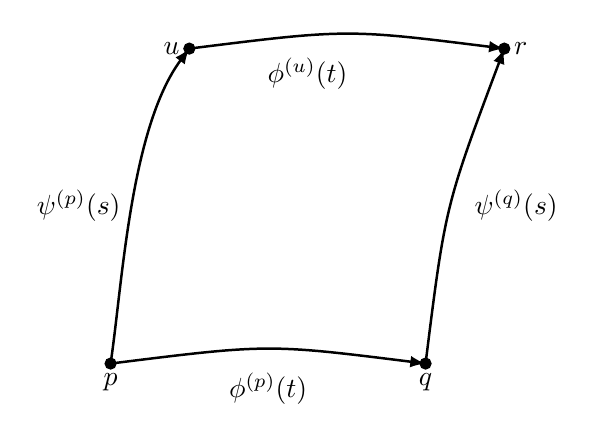
\begin{tikzpicture}
		
			\filldraw 
				(0,0) circle (2pt) node[align=left,   below] {$p$}
				(4,0) circle (2pt) node[align=center, below] {$q$}
				(1,4) circle (2pt) node[anchor=east] {$u$}
				(5,4) circle (2pt) node[anchor=west] {$r$};
			
			\draw [->, line width = 0.9pt] (0,0) .. controls(0.15,1) and (0.25,3) .. (1,4);
			\draw(0,0)[->,line width = 0.9pt] .. controls(2,0.25) .. (4,0);
			\draw (1,4)[->,line width = 0.9pt] .. controls (3,4.25) .. (5,4);
			\draw(4,0)[->,line width = 0.9pt] .. controls(4.25,2) .. (5,4);
			
			\draw
				(2,0) node[anchor=north] {$\phi^{(p)}(t)$}
				(0.25,2) node[anchor=east] {$\psi^{(p)}(s)$}
				(2.5,4) node[anchor=north] {$\phi^{(u)}(t)$}
				(4.5,2) node[anchor=west] {$\psi^{(q)}(s)$};
			
		\end{tikzpicture}
	\caption{Two alternate routes between points on a manifold via commuting flows. Here $r = \phi_{\delta t} \circ \psi_{\delta s}(p) = \psi_{\delta s} \circ \phi_{\delta t}(p)$.}
	\end{center}
\end{figure}

Let $v \in T_pM$, there are two ways we can translate this vector to $r$ via parallel transport, namely along the path $pur$, or the path $pqr$. Let $v' \in T_rM$ denote the result of the former transport, and $v'' \in T_rM$ the latter. Let $Z$ be any vector field defined in a neighbourhood of $p$ such that $Z\vert_p = v$, then.
	\begin{equation}
		\lim_{\delta s, \delta t \to 0} \frac{v'' - v'}{\delta s \delta t} = R(Z,X,Y)\vert_{p}.
	\end{equation}
	
\paragraph{Remark:} We shan't prove this lemma, but merely comment on it. In English, it essentially states that $R$ measures the 'rotation' of a vector under parallel transport. This formalises a fairly intuitive notion of curvature. Namely, if one imagines 'sliding' a tangent vector around on a sphere over a closed loop, they would see that the direction the arrow points at the end is \textit{not} the same as when it began. Specifically $R$ appears as we shrink any such loop down to a given point. This is all explored in more depth in the area of Differential Geometry known as \textit{Holonomy}. Here we can find results such as $R(X,Y)$ is an element of the Lie algebra of the holonomy group at $p$, and, for orientable Riemannian $n$-manifolds, the holonomy group is SO$(n)$, i.e. parallel transport must preserve the magnitude of the tangent vector, but nothing else.

\subsection{Symmetries of the Riemann Tensor}

\paragraph{} In a 4-dimensional spacetime, in a given basis the Riemann tensor has $4^4 = 256$ components. Surely not all of these are necessary to hold all of the data about the curvature of a connection? Thankfully, this is indeed not the case, given even a few basic assumptions, there are a lot of constraints that can be placed upon the Riemann tensor. One of which we have already seen and requires no assumptions. Namely, from the anti-symmetry inherent in the definition of the tensor, in abstract indices we can write
	\begin{equation}
		R^a_{b(cd)} = 0.
	\end{equation}
This immediately reduces the 16 degrees of freedom in the last indices down to 6\footnote{More generally, $n^2$ degrees of freedom are reduced to $\tfrac{1}{2}n(n-1)$.}, bringing the total to 96. In this section we will introduce a handful of other constraints one may impose on the Riemann tensor.

\paragraph{Lemma:} Let $(M,\nabla)$ be a smooth manifold with torsion-free connection. If $R^a_{bcd}$ is the resulting Riemann curvature tensor, then
	\begin{equation}
		R^a_{[bcd]} = 0.
	\end{equation}
	
\paragraph{Proof:} We shall prove the result holds in normal coordinates, then assert that it must hold true in any coordinate system. In normal coordinates, the Christoffel symbols at a point momentarily vanish, and so the components of the Riemann tensor reduce to
	\begin{equation}
		R^\mu_{\nu\rho\sigma}(p) = \left(\partial_\rho \Gamma^\mu_{\nu\sigma} - \partial_\sigma \Gamma^\mu_{\nu\rho} \right) \vert_p
	\end{equation}
\todo[inline]{Finish Proof}

\paragraph{Lemma:}\textit{(The Bianchi Identity)}

For $(M,\nabla), R^a_{bcd}$ as above,
	\begin{equation}
		R^a_{b[cd;e]} = 0.
	\end{equation}
	
\paragraph{Proof:}
\todo[inline]{Finish Proof}

\subsection{Geodesic Deviation}
\paragraph{} If we are dealing with a Riemannian manifold, we have a quick and easy way to (loosely) classify curvature. Namely, by observing the intersections of geodesics.

\paragraph{Examples:} Given a Riemannian manifold $(M,g)$, then any two geodesics
	\begin{enumerate}
		\item[Sphere:] Will always intersect at two distinct points. (Example of positive curvature)
		\item[Plane:] Will intersect at precisely one point, unless they are parallel, in which case no such intersection occurs, and the 'distance' between the lines is constant. (Example of no curvature)
		\item[Hyperbolic Plane:] Will always diverge if they originated from the same point. (Example of negative curvature)
	\end{enumerate}
	
\begin{definition}
	Let $(M,g)$ be a Riemannian manifold. A \textbf{1-parameter family of geodesics} is a map $\gamma: I \times I: \longrightarrow M$ such that
		\begin{itemize}
			\item $I$ and $I'$ are both open intervals of $\mathbb{R}$;
			\item For any fixed $s \in I$, $\gamma(s,t)$ is a geodesic on M with affine parameter $t$;
			\item The restriction of $\gamma$ to its image gives a diffeomorphism.
		\end{itemize}
\end{definition}

\paragraph{Remark:} Note that any open interval of $\mathbb{R}$ is diffeomorphic to $\mathbb{R}$ itself \todo{Finish Remark}

\paragraph{Proposition:} $\nabla_T \nabla_T S = R(T,S,T)$

\paragraph{Proof:} As the Levi-Civita connection is torsion-free, we have
	\begin{equation}
		\nabla_T S - \nabla_S T = [T,S] = 0.
	\end{equation}
Expanding out the definition of the curvature tensor, and again using the commutativity of the vector fields, we have
	\begin{align}
		R(T,S,T) &= \nabla_T \nabla_S T - \nabla_S \underbrace{\nabla_T T}_{=0},\\
						&= \nabla_T \nabla_T S. \qed
	\end{align}

\subsection{Curvature of the Levi-Civita Connection}

\paragraph{} Recall that the Levi-Civita connection is defined dependent on a metric [FINISH]

\paragraph{Proposition:} $R_{abcd} \left( := R^e_{bcd} g_{ae} \right) = R_{cdab}$ ; $R_{(ab)cd}=0$.

\paragraph{Proof:} \todo{Finish Proof}


\paragraph{Proposition:} The Ricci tensor of a Levi-Civita connection is symmetric.

\paragraph{Proof:} $R_{ab} = R^c_{acb} = g^{cd} R_{dacb} = g^{cd} R_{cbda} = R^d_{bda} = R_{ba}$. \qed

With a Levi-Civita connection, we can even "condense" our curvature tensor further, down to a scalar and still retain some useful information.

\begin{definition}
	Given a Riemannian manifold with Ricci tensor $R_{ab}$, the \textbf{Ricci scalar} is defined by
		\begin{align}
			R := g^{ab} R_{ab},
		\end{align}
\end{definition}

\paragraph{Remark:} Remarkably, for a 2-manifold embedded in $\mathbb{R}^3$, this definition coincides with the classical Gaussian curvature!

\chapter{The Einstein Equations}

\paragraph{} Finally we arrive at the culmination of the first part of the course, the equations of General Relativity themselves, the Einstein equations. After one last definition:

\begin{definition}
	The \textbf{Einstein tensor} of a Riemannian manifold is defined by
		\begin{align}
			G_{ab} := R_{ab} - \tfrac{1}{2} g_{ab} R.
		\end{align}
\end{definition}

\paragraph{Remark:} The Einstein tensor can be said to be divergence-free, according to the equation
	\begin{align}
		g^{ac} \nabla_c G_{ab} =: \nabla^a G_{ab} = 0.
	\end{align}
	
\paragraph{} Originally, the equation that Einstein wrote was
	\begin{align}
		G_{ab} = \frac{8 \pi G}{c^4} T_{ab}.
	\end{align}
His first guess included only the Ricci tensor on the left hand side, however, the conservation of energy and momentum requires that the tensor on the right (the \textit{energy-momentum tensor}) be divergence free. The addition of the Ricci scalar term ensures this condition is also met on the left. In Einstein's own words, the left hand side of this equation is a "marble palace", referring to entirely geometric entities. And the right is a "wooden shed", consisting of a "source-term" encoding the distribution of matter throughout spacetime, however inelegant that may be.

\paragraph{} Unfortunately, this equation is in fact in disagreement with experiment. What is missing is an explanation of the apparent expansion of the universe. Mathematically this appears in the equation as a contribution of the form
	\begin{align}
		G_{ab} + \Lambda g_{ab} = \frac{8 \pi G}{c^4} T_{ab}.
	\end{align}
Where $\Lambda$ is the infamous cosmological constant, which so far has not been predicted by any theory to even a remote degree of accuracy.

\paragraph{} Ignoring the cosmological `bodge' for now, in a vacuum the energy-momentum tensor vanishes by definition. Thus the Einstein equations are simply $G_{ab} = 0$. A little algebra shows us that this implies $R = 0$, which further implies that each component of the Ricci tensor vanishes. In normal coordinates one can (perhaps???) express this as
	\begin{align}
		R_{\mu \nu} = R^\rho_{\mu \rho \nu} = g^{\rho \sigma} \left( \partial_{\mu} \partial_{[\rho} g_{\nu] \sigma} - \partial_\sigma \partial_{[\rho} g_{\nu] \mu} \right) = 0.
	\end{align}
This is a second order non-linear system of PDEs, and is sufficiently messy that to this day full solutions are not yet known.

\todo[inline]{Preamble to Einstein manifolds}

\begin{definition}
	Let $(M,g)$ be a Riemannian manifold of dimension $n$. If ${R_{ab} = \tfrac{1}{n} R g_{ab}}$, then we say it is an \textbf{Einstein manifold}.
\end{definition}

\paragraph{Lemma:} The degrees of freedom afforded by the dimensionality of a manifold constrain the curvature in the following ways
	\begin{itemize}
		\item For $n = 2$, \textit{any} metric is Einstein
		\item For $n = 3$, the Riemann tensor is completely determined by the Ricci tensor. Furthermore, the Ricci tensor satisfies the Einstein condition above if and only if the space has constant curvature; the space is then locally diffeomorphic to one of: flat space, a 3-sphere, hyperbolic space.
		\item For $n \geq 4$, the Riemann tensor can be expressed in a form isolating the degrees of freedom as
			\begin{equation}
				R_{abcd} = \underbrace{C_{abcd}}_{\text{The }\textit{Weyl tensor}} + \tfrac{2}{n-2} \left(g_{a[c} R_{d]b} - g_{b [c} R_{d] a} \right) - \tfrac{2}{(n-1)(n-2)}R g_{a [c} g_{d] b}.
			\end{equation}
	\end{itemize}

\paragraph{Remark:} We shan't prove any of these results, but we will make a few comments on the Weyl tensor. It is traceless in all its indices, so contracting any two of its indices with the metric will give $0$. Roughly speaking, the Riemann tensor for a Lorentzian manifold measures the tidal forces acting on a body. More specifically the Ricci tensor measures exactly how the volume of an object changes in the presence of such forces, therefore the Weyl tensor quantifies all aspects of the tidal force that distort the shape, but says nothing about the volume. It is also invariant under a group of transformations known as the \textit{conformal group}. If the Weyl tensor vanishes, then one can find such a conformal transformation that the metric is flat - in which case we say the manifold is \textit{conformally flat}.

\section{Examples}

\todo[inline]{Intro}

\subsection{Schwarzshild Metric}

\paragraph{} One of the first solutions to the Einstein equations, the Schwarzschild metric describes a universe containing nothing but an eternal, stationary black hole - thus it is a vacuum solution, satisfying $R_{ab} = 0$. It is conventionally written as
	\begin{equation}
		g = \left( 1 - \tfrac{2m}{r} \right)dt^2 + \left( 1 - \tfrac{2m}{r} \right)^{-1} dr^2 + r^2 \left( d\theta^2 + \sin^2\theta d\phi^2 \right).
	\end{equation}
	
\paragraph{Remark:} Immediately, one will notice that there are two values of $r$ for which this metric is not defined. The \textit{singularities} occur at $r = 2m$, and $r = 0$. It turns out that the first of these can be ignored by simply changing coordinates, whereas the second is more insidious. In general it is difficult to ascertain which singularities of a metric are coordinate singularities, and which are "genuine". In this case, a hint that the latter is more serious is the fact that $R^{abcd}R_{abcd} = \tfrac{1}{r}$.

\subsection{The n-sphere}

\paragraph{} A simple metric, and somewhat intuitive. Consider the $n$-sphere, $S^n$, embedded in $\mathbb{R}^{n+1}$. It has a Riemannian metric given by the restriction of the Euclidean metric on $\mathbb{R}^{n+1}$, which gives rise to the following features of curvature
	\begin{align}
		R_{ab} = \tfrac{1}{n} R g_{ab} ;  \quad C^a_{bcd} = 0,
	\end{align}
where $R$ is any positive constant.

\subsection{The pp wave}

\paragraph{} In the local coordinates $(x,y,u,v)$ we have the metric
	\begin{equation}
		g = dx^2 + dy^2 + du dv + H(u,x,y) du^2.
	\end{equation}
Here, $H(u,x,y)$ is an arbitrary function. In a vacuum, the condition $R_{ab} = 0$ implies that $H_{xx} + H_{yy} = 0$, i.e. $H$ is harmonic in the first two coordinates.

\chapter{Into Non-Riemannian Geometries}

\section{Newton-Cartan Geometries}

\paragraph{} The language of Differential Geometry is both versatile and powerful. As one may expect, we can recast Newtonian gravity as a geometric theory. However, the result is in fact more complicated than General Relativity! First, we begin with a standard equation of Newtonian physics, writing the acceleration of a particle due to a gravitational potential
	\begin{equation}\label{NewtGrav}
		\ddot{\mathbf{x}} = -\boldsymbol{\nabla} \Phi.
	\end{equation}
We wish to find a theory such that this is the result of the geodesic equation for some connection. The manifold upon which the laws of Newtonian physics play out is still inherently 4-dimensional so we will use the same coordinates as usual, $(x^\mu)$, where $x^0 = t$. Recall the geodesic equation \eqref{Geodesic} is
	\begin{equation}
		\ddot{x}^\mu + \Gamma^\mu_{\nu\rho} \dot{x}^\nu \dot{x}^\rho = 0.
	\end{equation}
In our chosen coordinates the connection is defined through the Christoffel symbols as
	\begin{equation}
		\Gamma^i_{00} = \delta^{ij} \tfrac{\partial}{\partial x^j} \Phi, \quad \Gamma^\mu_{i0} = \Gamma^\mu_{0i} = 0.
	\end{equation}
From here it is easy to verify that \eqref{Geodesic} recovers \eqref{NewtGrav}.

\todo[inline]{Some lead up}

\begin{definition}
	A \textbf{Newton-Cartan structure} on an $n$-manifold $M$ is a tuple $(h,\theta,\nabla)$, where
		\begin{enumerate}[label=(\roman*)]
			\item $h$ is a degenerate, symmetric, type $(2,0)$ tensor,
			\item $\theta$ is a $1$-form in the kernel of $h$, i.e. $h^{ab} \theta_b = 0$,
			\item $\nabla$ is a torsion-free connection preserving both $h$ and $\theta$, i.e. $\nabla_a h^{bc} = \nabla_a \theta_b = 0$.
		\end{enumerate}
\end{definition}

\paragraph{Remark:} [de-Rham cohomology implies that $\theta = dt$ is unique up to addition of a constant]. [Also, 'universal clock' $\tau: M \longrightarrow \mathbb{R}$].
\todo[inline]{Flesh out remark}

\section{Projective Structures}

\todo[inline]{Intro}

\begin{definition}
	Two torsion-free connections are \textbf{projectively equivalent} if they solve the same \textit{unparametrised geodesics}
\end{definition}

\todo[inline]{[GIVE DETAILED EXAMPLE]}

\paragraph{Claim:} Two torsion-free connections, $\nabla$ and $\widehat{\nabla}$, on $TM$  are projectively equivalent if there exists $\omega \in \Omega^1(M)$ such that
	\begin{align}
		\widehat{\Gamma}^\mu_{\nu\rho} = \Gamma^\mu_{\nu \rho} + \delta^\mu_\nu \omega_\rho + \delta^\mu_\rho \omega_\nu.
	\end{align}
	
\paragraph{Proof:}

\todo[inline]{[GIVE PROOF]}

\paragraph{Example:} [Mapping between geodesics in stereographic projection (based at centre of half sphere though)]
\todo[inline]{Flesh out example}

\section{Magnetic Geometries and Kaluza-Klein Reductions}

\paragraph{} Consider the Riemannian manifold $(\mathbb{R}^3,g)$, where
	\begin{align}
		g = dx^2 + dy^2 + (dz - xdy)^2.
	\end{align}
The Lagrangian for the geodesic equation is then
	\begin{align}
		\mathcal{L} = \tfrac{1}{2} \dot{x}^2 + \tfrac{1}{2} \dot{y}^2 + \tfrac{1}{2}(\dot{z} - x\dot{y})^2.
	\end{align}
	
\paragraph{Exercise:} By considering the symmetries of the Lagrangian, show that the geodesics of this metric are circles.

\paragraph{} The [Got lost here... show how this arises from the given curvature form]
\todo{Finish Example}

\chapter{Physical Laws on Curved Spacetime}

\section{Equivalence Principles}

\paragraph{} We shall now briefly return to physical laws, and used our new mathematical background to attempt to generalise these to a curved spacetime. In order to find the correct process for abstracting physical laws, we need to return to the fundamental observations underlying the theory of General Relativity. The \textit{equivalence principles}.

\paragraph{} As he may have written them, two of Isaac Newton's most famous equations read
	\begin{equation}\label{eq:NewtonsLaws}
		\mathbf{F} = \dot{\mathbf{p}}; \quad \mathbf{F} = - G \frac{m M}{r^2}\hat{\mathbf{r}}. 
	\end{equation}
The equation on the left is Newton's second law of motion. Originally, Newton only made reference to the momentum of a body, stating that it changed at a rate proportional to the force. Then a further observation was made that the momentum of a body is proportional to its velocity, with the constant of proportionality being the \textit{inertia} of the body. Considered in isolation from this, the latter equation, the law of gravitation, simply exemplifies one such force that may give rise to this change in momentum. The two `$m$' terms appearing in this equation act as a gravitational \textit{charge}, determining both the extent to which one body exerts an influence, and how sensitive a second body is to that influence. Put differently, the more massive a body, the greater its ability to pull, and the greater the pull it experiences in relation to any other body.

\paragraph{} If we make two substitutions, $\mathbf{p} = m_I \dot{\mathbf{x}}$ and $\mathbf{g} = - G\tfrac{M}{r^2}\hat{\mathbf{r}}$, we see the effect of the gravitational force as written is
	\begin{align}
		\ddot{\mathbf{x}} = \frac{m}{m_I} \mathbf{g}.
	\end{align}
Here is the strange coincidence, and we should really stress, that before the 20\textsuperscript{th} century, there was \textit{no} theoretical explanation for this: as far as the most accurate experiments to date have measured, the quotient on the right hand is $1$. The consequence of this is that the trajectory of a body in a gravitational field $\mathbf{g}(\mathbf{x})$, is determined uniquely by just an initial position and velocity, with \textit{no} dependence on any properties the body may posses. This makes gravity unique amongst all laws of physics, whereas every other known interaction is modified by certain characteristics of the bodies involved, gravity is universally ambivalent. This, is known as the \textit{weak equivalence principle}, and can be summarised as $m_I = m$.

\paragraph{}
The interpretation of this principle involving trajectories is particularly enlightening.
We shall make a generalisation of the gravitational law (\ref{eq:NewtonsLaws}b) by considering a distribution of mass (excluding the test object) throughout space given by a density function $ \rho(\mathbf{y}) $.
The equation of motion describing this trajectory, assuming the weak equivalence principle is then
	\begin{equation}\label{key}
		\ddot{\mathbf{x}}(t) = \int_{\mathbb{R}^3} \frac{G\rho(\mathbf{y})}{|\mathbf{y}-\mathbf{x}(t)|^3} \left(\mathbf{y} - \mathbf{x}(t)\right) \mathrm{d}^3y.
	\end{equation}
If we assume the density function $ \rho $ to be constant, then this presents an initial value problem whose solutions are determined \textit{uniquely} by the initial data $ \mathbf{x}(0) $, $ \dot{\mathbf{x}}(0) $. Importantly, this does not depend on any of the \textit{physical} characteristics of the test object. This leads to an alternative formulation of the weak equivalence principle:
	\begin{displayquote}
		The trajectory of a free falling test body depends only on its initial position and velocity; it is independent of its composition.
	\end{displayquote}

\paragraph{}
Moreover, if we can take the gravitational field at $ \mathbf{x} $ to be constant (i.e. $ \rho $ has support in a region far away from $ \mathbf{x} $), then $ \ddot{\mathbf{x}} = \mathbf{g} $ for some constant vector $ \mathbf{g} $.
Consider an entire laboratory which follows this trajectory. Let $ \mathbf{z} $ denote the position of a test particle in an intertial frame, then in the lab frame $ \mathbf{z}' = \mathbf{z} - \mathbf{x} \Rightarrow \ddot{\mathbf{z}} = \ddot{\mathbf{z}} - \ddot{\mathbf{x}} = \mathbf{g} = \mathbf{g} = 0 $, i.e. observers in the laboratory do not observe the test particle to be in a gravitational field.
Note this result only holds for a \textit{contant} gravitational field. We shall study later how a varying gravitational field leads to the observation of \textsl{tidal forces} in the lab frame.

\paragraph{}
Reference frames such as the one of our laboratory in the above example are often useful in GR.
As such, we refer to them as \textsl{locally inertial frames} (\textsc{lif}s), a precise definition of which will be given later on.
For now though, we can think of \textsc{lif}s as the Lorentzian equivalent of normal coordinates, where the metric $ g $ is instantaneously stationary at some point $ p $ in the chart.

\paragraph{}
The notion of equivalence that will allow us to begin deriving curved spacetime analogs of existing physical laws is the following, due to Einstein:
	\begin{itemize}
		\item The weak equivalence principle from above holds, also
		\item In a \textsc{lif}, all non-gravitational experiments will be indistinguishable from those performed in an inertial frame in Minkowski space.
	\end{itemize}

\section{Minimal Coupling}

\paragraph{}
Our aim is to generalise laws defined on a Minkowski spacetime to laws on any Lorentzian manifold.
One procedure which achieves this whilst also satisfying the Einstein equivalence principle is known as \textsl{minimal coupling}, and can be expressed mathematically as
	\begin{enumerate}
		\item $ \eta_{\mu\nu} \mapsto g_{\mu\nu} $,
		\item $ \partial_\mu \mapsto \nabla_\mu $,
		\item $ \mu, \nu, \cdots \mapsto a, b, \cdots $.
	\end{enumerate}

\paragraph{}
In words, we first replace any occurrence of the Minkowski metric $ \eta $ with a generally curved metric $ g $.
Next we replace any partial derivatives with covariant derivatives.
As the Christoffel symbols which define the covariant derivative are dependent on the \textit{derivatives} of the metric, if the metric is stationary at a point, then all the Christoffel symbols will vanish and the covariant derivative will coincide with the partial derivatives.
Finally, as long as we are sure that the equation thus obtained transforms tensorially, we can transition to a coordinate free equation by simply replacing the greek indices with abstract indices.

\begin{example}[Klein-Gordon Equation]
	Perhaps the simplest law to generalise to a curved spacetime is the Klein-Gordon field equation for a field of mass $ m $:
	\begin{equation*}\label{key}
	\left( \eta_{\mu \nu} \partial^\mu \partial^\nu - m^2 \right) \Phi = 0 \mapsto \left( g_{ab} \nabla^a \nabla^b - m^2 \right) \Phi = 0.
	\end{equation*}
\end{example}

\begin{example}[Electromagnetism]
	Firstly, we need to generalise the definition of the electromagnetic field strength tensor as
		\begin{equation}\label{key}
			F_{ab} = \nabla_{[a} A_{b]}.
		\end{equation}
	Then we can write the curved spacetime form of Maxwell's equations as
		\begin{equation}\label{key}
			\nabla_a F^{ab} = 0; \quad \nabla_{[a} F_{bc]} = 0.
		\end{equation}
	To represent the interaction of this field with matter, we must generalise the Lorentz force law $ \mathbf{F} = q (\mathbf{E} + \mathbf{v} \times \mathbf{B} ) $. Recall that if $ \tau $ is the proper time along the trajectory of a particle, then $ \tfrac{d}{d\tau} = \nabla_u $, where $ u = \tfrac{dx}{d\tau} $ is the 4-velocity of the particle. From here, one can then show that, under minimal coupling, the Lorentz force law becomes
		\begin{equation}\label{key}
			\nabla_u u^a = \frac{q}{m} F^a_b x^b.
		\end{equation}
\end{example}

\paragraph{}
Following the procedure for minimal coupling in reverse, we can verify that the generalisations offered in both examples do indeed coincide with their Minkowskian equivalents.
However, one thing we must bear in mind is that we cannot expect this procedure to give us \textit{all} possible physical laws, as it is perfectly reasonable to suppose that there may be laws which `vanish', or become trivial in some way, in a locally inertial frame.

\end{document}
